%!TEX root = ../PhD_thesis__Lilian_Besson

% First chapter begins here
\chapter{Single Player and Stationary Multi-Armed Bandit Models}
\label{chapter:2}
\minitoc

Abstract for Chapter 2.

\newpage
% Write miniTOC just after the title
\graphicspath{{2-Chapters/2-Chapter/Images/}}

% ----------------------------------------------------------------------------
\section{Stationary MAB models}
\label{sec:2:notations}

% ----------------------------------------------------------------------------
\subsection{Finite arms and stochastic rewards}

In this thesis, we only consider models with finite arms.
No linear bandits, no contextual bandits etc.

For now, we only consider stochastic rewards. Piece-wise stochastic models are studied in Chapter~\ref{chapter:6}.


% ----------------------------------------------------------------------------
\subsection{Different hypotheses on rewards distributions}

Everything is implemented and documented at
https://smpybandits.github.io/docs/Arms.html

Bernoulli, Gaussian, sub-Bernoulli, sub-Gaussian, Exponential, sub-Exponential...

One dimensional exponential family...

Just bounded, in $[a,b]$ but without loss of generality in $[0,1]$ etc.

Markov models: presented later in Section~\ref{sec:3:markovModels}.


% ----------------------------------------------------------------------------
\section{Applications of stationary MAB}
\label{sec:2:applicationsofStationaryMAB}

\subsection{Various possible applications}

- clinical trial
- A/B testing of websites
- online content recommandation
- wireless communication, lots of possibilities, one is frequency/channel selection in the OSA paradigm, detailed after
- hyper-parameters tuning of deep neural networks etc


\subsection{Application for Opportunistic Spectrum Access}

Detail the analogy arm = channel in a licensed spectrum, rewards $r_k(t)$ = 1 if no Primary User or 0 if channel $k$ is busy at time $t$.

Detail the previous work from our team SCEE on bandits + OSA : Wassim, Navik


% ----------------------------------------------------------------------------
\section{Review of MAB algorithms}
\label{sec:2:famousMABalgorithms}

Everything is implemented and documented at
https://smpybandits.github.io/docs/Policies.html


\subsubsection{Why do we need smart algorithms?}
Why Follow-the-Leader (EmpiricalMeans https://smpybandits.github.io/docs/Policies.EmpiricalMeans.html) don't work, example.

\subsection{Simple but efficient algorithms when well tuned: $\varepsilon$-greedy and Explore-then-Commit}

See
https://smpybandits.github.io/docs/Policies.EpsilonGreedy.html
https://smpybandits.github.io/docs/Policies.ExploreThenCommit.html


% ----------------------------------------------------------------------------
\subsection{Index policies: UCB and others}

\subsubsection{UCB}
Optimism in face of uncertainty, for UCB etc.


\subsubsection{klUCB}
Optimal upper confidence bounds based on Kullback-Leibler divergence and klUCB indexes

\subsubsection{Other policies inspired by UCB}

- UCB-H and klUCB-H
- UCB-V
- UCB-dagger
- UCBoost
- UCB+ and klUCB+


% ----------------------------------------------------------------------------
\subsection{Bayesian policies: Thompson Sampling and others}

Idea behind Thompson sampling and Bayesian philosophy.

The Beta posterior and others (https://smpybandits.github.io/docs/Policies.Posterior.html) and Thompson Sampling.


% ----------------------------------------------------------------------------
\subsection{Other policies: BESA and others}

It's a good opportunity to show off and say that I worked on my own on some non-standard policies.

- One of the first paper I read in 2016 was defining AdBandits, https://smpybandits.github.io/docs/Policies.AdBandits.html, a mixture between Thompson sampling and BayesUCB (very efficient in practice)
- I especially love the BESA algorithm by [? and ? and Maillard].


% ----------------------------------------------------------------------------
\subsection{Policies for adversarial bandits: Exp3 and others}

Exp3, Exp3++ etc
https://smpybandits.github.io/docs/Policies.Exp3.html
https://smpybandits.github.io/docs/Policies.Exp3PlusPlus.html

Softmax: is it the same, but written differently?
https://smpybandits.github.io/docs/Policies.Softmax.html


% ----------------------------------------------------------------------------
\subsection{Hybrid policies: MOSS, klUCB++ and klUCB-Switch and others}

Recent work.
https://smpybandits.github.io/docs/Policies.MOSS.html
https://smpybandits.github.io/docs/Policies.IMED.html
https://smpybandits.github.io/docs/Policies.klUCBPlusPlus.html
https://smpybandits.github.io/docs/Policies.klUCBSwitch.html

Talk about these?
https://smpybandits.github.io/docs/Policies.OCUCB.html
https://smpybandits.github.io/docs/Policies.OSSB.html

With perturbation: maybe we don't need optimism in face of uncertainty, we just need uniform sampling!
Randomized Confidence Bound (RCB) with uniform perturbations performs as well as UCB!
https://smpybandits.github.io/docs/Policies.RandomizedIndexPolicy.html


\subsection{Summary of classification of the most famous algorithms}

A huge table in one page in portrait mode, giving:
- name
- reference, year
- family, classification
- time/memory complexity ?
- regret bound for stochastic regret

of about 20/30 algorithms?


% ----------------------------------------------------------------------------
\section{Lower and upper bounds on regret}
\label{sec:2:lowerUpperBoundsRegret}


\subsection{Measuring performance with the (mean) regret}
Explain what is regret


\subsection{Regret lower bounds: do not detail too much, don't explain the tools behind the results}

- [Lai and Robbins] lower-bound in $\Omega(\log(T))$
- Worst case lower-bound in $\Omega(\sqrt{T})$
- Adversarial lower-bound in $\Omega(\sqrt{T})$ (also useful for piece-wise stationary models)


\subsection{Regret upper bounds, tools and different kinds of bounds}

- useful decomposition, with number of samples (see Claire's PhD)
- different kinds of bounds, problem-dependent with $\bigO{C \log(T)}$ with $C$ a measure of the problem complexity, or problem-independent with $\bigO{\sqrt{KT}}$ ?
- tools to show regret upper-bounds, concentration inequalities,
- short proof of UCB or klUCB? just to start to show the tools


\subsection{Other measures of performances}

- Quantile regret or just histogram of regrets
- Worst case regret (max $R_T^{r}$ for $r$ index of Monte-Carlo simulation?)
- Fairness


% ----------------------------------------------------------------------------
\section{Different approaches on algorithm selection}
\label{sec:2:chooseYourPreferredBanditAlgorithm}

\subsection{Naive approach: use UCB or Thompson sampling, and forget about the rest!}
First solution: be naive, only use UCB everywhere

\subsection{Use prior knowledge about the future application to select beforehand the chosen algorithm}
Second solution, if one has some prior knowledge about the domain or setting for which the learning algorithms will be deployed, she can run synthetic or real-world simulations, compare many algorithms before deployment, and select the best algorithm!

\subsection{Online algorithm selection with expert aggregation}

% - ``Aggregation of Multi-Armed Bandits learning algorithms for Opportunistic Spectrum Access'', see https://hal.inria.fr/hal-01705292

As we said, a third possible approach is to select \emph{on the run} the best algorithm for a specific situation, for which the so called \emph{expert aggregation algorithms} framework can be useful.
%
To the best of our knowledge, aggregation algorithms, such as \ExpQ{} which dates back from 2002 \cite{Auer02},
have never been used in pratice for stochastic MAB problems.
% and we show that it appears empirically sub-optimal when applied to simple stochastic problems.

We present an improved variant of \ExpQ, called \Aggr.
For synthetic MAB problems, with Bernoulli or other distributions for $K$ arms, simulation results are presented to demonstrate its empirical efficiency.
We combine classical algorithms, such as Thompson sampling, Upper-Confidence Bounds algorithms (\UCB{} and variants), and Bayesian or Kullback-Leibler UCB.
%
Our algorithm offers good performance compared to state-of-the-art algorithms
(\ExpQ{}, \CORRAL{} or \LearnExp{}) \cite{Agarwal16,Singla17},
and appears as a robust approach to select on the run the best algorithm for any stochastic MAB problem, being more realistic to real-world radio settings than any tuning-based approach.

% \TODOL{This chapter is basically a raw include from my paper ``Aggregation of Multi-Armed Bandits learning algorithms for Opportunistic Spectrum Access'', see https://hal.inria.fr/hal-01705292}


% ----------------------------------------------------------------------
% \subsection{Aggregating bandit algorithms}\label{sub:25:aggregation}
\paragraph{Notations}\label{sub:25:aggregation}

We assume to have $N \geq 2$ MAB algorithms, $\Alg_1, \dots, \Alg_N$,
and let $\Alg_{\mathrm{aggr}}$ be an aggregation algorithm,
which runs the $N$ algorithms in parallel (with the same slotted time), and use them to choose its channels based on a voting from their $N$ decisions.
%
$\Alg_{\mathrm{aggr}}$ depends on a pool of algorithms and a set of parameters.
We would like that $\Alg_{\mathrm{aggr}}$
performs almost as well as the best of the $\Alg_a$, with a good choice of its parameters, independently of the MAB problem.
Ideally $\Alg_{\mathrm{aggr}}$ should perform similarly to the best of the $\Alg_a$.
%
To simplify the presentation, we only aggregate bandit algorithms that give deterministic recommendations:
one arm is chosen with probability $1$ and the others with probability $0$.
However, both \ExpQ{} and \Aggr{} can be adapted to aggregate randomized bandit algorithms, \ie, algorithms that output a probability distribution $\xi_t$ over the arms $[K]$ at each time step, and draw the next selected arm according to this distribution
(\eg, Thompson sampling).

The aggregation algorithm maintains a probability distribution $\pi^{t}$ on the $N$ algorithms $\Alg_a$, starting from a uniform distribution:
$\pi^t_a$ is the probability of trusting the decision made by algorithm $\Alg_a$ at time $t$.
$\Alg_{\mathrm{aggr}}$ then simply performs a weighted vote on its algorithms: it decides whom to trust by sampling $a \in [N]$ from $\pi^t$, then follows $\Alg_a$'s decision.
The main questions are then to know what observations (\ie, arms and rewards) should be given as feedback to which algorithms,
and how to update the trusts at each step, and our proposal \Aggr{} differs from \ExpQ{} on these very points.


% ----------------------------------------------------------------------
\subsection{Our contribution: the \Aggr{} algorithm}\label{sub:25:Aggr}

Our proposed \Aggr{} is detailed in Algorithm~\ref{algo:25:Aggr}.
%
\begin{small}
	\begin{figure}[h!]
		\centering
		\begin{framed}
		% Documentation at http://mirror.ctan.org/tex-archive/macros/latex/contrib/algorithm2e/doc/algorithm2e.pdf if needed
		% Or https://en.wikibooks.org/wiki/LaTeX/Algorithms#Typesetting_using_the_algorithm2e_package
		\begin{algorithm}[H]
			% XXX Input, data and output
			\KwIn{$N$ bandit algorithms, $\Alg_1, \dots, \Alg_N$, with $N \geq 2$}
			\KwIn{Number of arms, $K \geq 2$}
			\KwIn{Time horizon, $T \geq 1$, \textbf{not} used for the learning}
			\KwIn{A sequence of learning rates, $(\eta_t)_{t \geq 1}$}
			\KwData{Initial uniform distribution, $\pi^{0} = \cU([N])$}
			\KwResult{$\Alg_{\mathrm{aggr}}=\Aggr\left[\Alg_1, \dots, \Alg_N\right]$}
			% XXX Algorithm
			\For(\tcp*[f]{At every time step})
            {$t = 1, \dots, T$}{
				%
				% \tcp{First, run each algorithm $\Alg_a$}
				\For(\tcp*[f]{Can be parallel}){$a = 1, \dots, N$}{
					$\Alg_a$ updates its internal state (e.g., \UCB{} indexes)\;
					It chooses $A(t+1)_{a} \in [K]$.
				}
				%
				% \tcp{The more algorithms have chosen arm $j$, the more probable it is to be chosen.}
				Let $p^{t+1}_j := \sum\limits_{a = 1}^{N} \pi^{t}_a \times \mathbbm{1}(\{A(t+1)_{a} = j\}), \;\forall 1\leq j \leq K$\;
				% \tcp*{Sum trusts}
				Then $\Alg_{\mathrm{aggr}}$ chooses arm $A(t+1) \sim p^{t+1}$\;
				% $\P(A(t+1)_{\mathrm{aggr}} = j) = p^{t+1}_j$
				% \tcp*{Sample once}
				%
				Give \emph{original} reward $(A(t+1), 1 - \ell_{A(t+1)}(t+1))$ to \emph{each} $\Alg_a$ (maybe \emph{not} on its chosen arm)\;
				Compute an \emph{unbiased} estimate of the loss of the trusted algorithms,$$ \ell^{t+1} = \ell_{A(t+1)}(t+1) / p^{t+1}_{A(t+1)}\;. $$
				% \tcp{Use bandit feedback to update $\pi^{t}$}
				% \tcp{Finally, use the instantaneous bandit feedback (loss $\ell_{A(t+1),t}$) to update $\pi^{t}$}
				% \For(\tcp*[f]{Can be parallel}){$a = 1, \dots, N$}{
				\For{$a = 1, \dots, N$}{
					% \eIf{$\Alg_a$ was trusted, \ie, $A(t+1)_{a} = A(t+1)$}{
					\If{$\Alg_a$ was trusted, \ie, $A(t+1)_{a} = A(t+1)$}{
						$ \pi^{t+1}_{a} = \exp(\eta_t \ell^{t+1}) \times \pi^{t}_{a} $
						% \tcp*{More trusted}
						}%{
						% $ \pi^{t+1}_{a} = \exp(- \eta_t \ell^{t+1}) \times \pi^{t}_{a} $
						% \tcp*{Less trusted}
					% }
				}
				Renormalize the new $\pi$: $\pi^{t+1} := \pi^{t+1} / \sum_{a=1}^{N} \pi^{t+1}_{a}$.
				% \tcp*{Project it back to $\Delta_N$}
			}
			\caption{Our aggregation algorithm \Aggr.}
			\label{algo:25:Aggr}
		\end{algorithm}
		\end{framed}
	\end{figure}
\end{small}


At every time step, after having observed a loss $\ell_{A(t+1)}(t+1)$ for its chosen action $A(t+1)$,
the algorithm updates the trust probabilities from $\pi^t$ to $\pi^{t+1}$ by
a multiplicative exponential factor (using the learning rate and the \emph{unbiased} loss).
%
Only the algorithms $\Alg_a$ who advised the last decision get their trust updated, in order to trust more the ``reliable'' algorithms.

The loss estimate is unbiased in the following sense. If one had access to the rewards $r_k(t+1)$ (or the losses $\ell_k(t+1)$) for all arms $k$, the loss incurred by algorithm $a$ at time $t+1$ would be $\tilde{\ell}_{a,t+1} = \ell_{A_A(t+1)}(t+1)$. This quantity can only be observed for those algorithms for which $A_{a}^{t+1}=A(t+1)$. However, by dividing by the probability of observing this recommendation, one obtains an unbiased estimate of $\tilde{\ell}_{a,t}$. More precisely, if we define the estimate by
\begin{equation}
	\hat{\ell}_{a,t+1} = \frac{\ell_{A_A(t+1)}(t+1)}{p_{A_A(t+1)}^{t+1}} \mathbbm{1}(A_A(t+1) = A(t+1))
\end{equation}
satisfies $\mathbb{E}[\hat{\ell}_{a,t+1} | \mathcal{H}_t] = \tilde{\ell}_{a,t+1}$, for all $a$, where the expectation is taken conditionally to the history of observations up to round $t$, $\mathcal{H}_{t}$. Observe that $\tilde{\ell}_{a,t+1}=\ell^{t+1}$ for all algorithms $a$ such that $A_A(t+1)=A(t+1)$, and $\tilde{\ell}_{a,t+1}=0$ otherwise.


% - Precise some tricky points
An important feature of \Aggr{} is the feedback provided to each underlying bandit algorithm, upon the observation of arm $A(t+1)$. Rather than updating only the trusted algorithms (that is the algorithms which would have drawn arm $A(t+1)$) with the observed reward $r_{A(t+1)}(t+1)=1 - \ell_{A(t+1)}(t+1)$,  we found that updating each algorithm with the (original) loss observed for arm $A(t+1)$ improves the performance drastically.
%
As expected, the more feedback they get, the faster the underlying algorithms learn, and the better the aggregation algorithm is.
This intuition is backed up by theory explained in \cite{Maillard11}.


Regarding the update of $\pi^t$, one can note that the trust probabilities are not all updated before the normalization step,
and an alternative would be to
increase $\pi_{a}$ if $A(t+1)_a = A(t+1)$ and to decrease it otherwise.
It would not be so different, as there is a final renormalization step, and empirically this variation has little impact on the performance of \Aggr{}.



% ----------------------------------------------------------------------
\subsubsection{Explanations of \Aggr{} versus \ExpQ{} }\label{sub:25:Exp4}

% - explain, but don't give pseudo-code ?
The \ExpQ{} algorithm (see, e.g. \cite[Section 4.2]{Bubeck12})
is similar to \Aggr{}, presented in Algorithm \ref{algo:25:Aggr},
but differs in the two following points.
%
First, $a\sim\pi^t$ is sampled first and the arm chosen by $\Alg_a$ is trusted, whereas \Aggr{}
needs to listen to the $N$ decisions to perform the updates on $\pi^{t+1}$.
Then, \ExpQ{} gives back an observation (arm, reward) only to the last trusted algorithm
whereas \Aggr{} gives it to all algorithms.
%
Second, after having computed the loss estimate $\ell$, \ExpQ{} updates the estimated cumulative loss for each algorithm,
$\widetilde{L}_a(t) = \sum_{s=1}^{t} \ell_{A_a^s}(s) \times \mathbbm{1}(A^{s}_{a} = A^{s}_{\mathrm{aggr}})$.
%
Instead
\footnote{~It is the same for constant learning rates, and does not differ much for decreasing learning rates.}
of updating $\pi^{t}$ multiplicatively as we do for our proposal, \ExpQ{} recomputes it, proportionally to
$\exp(- \eta_t \widetilde{L}_a(t))$.


\paragraph{How to choose the learning rates $(\eta_t)$?}
%
The sequence of non-negative learning rates $(\eta_t)_{t \geq 1}$ used by \ExpQ{} can be arbitrary.
It can be constant but should be non-increasing \cite[Theorem 4.2]{Bubeck12}.
% helps to choose a good sequence.
If the horizon $T$ is known (and fixed), the best choice is given by $\eta_t = \eta = 2 \log(N) / (T K)$.
However, for real-world communication problems, it can be considered unrealistic\footnote{~For more discussion on this hypothesis, we refer to Section~1 of our article \cite{Besson2018DoublingTricks}.} to assume a fixed and known time horizon, so we prefer the alternative horizon-free choice%
\footnote{~It is non-increasing, and is obtained by minimizing the upper-bound on the regret derived in \cite[pp48]{Bubeck12}.}
of learning rates,
$\eta_t = \log(N) / (t K)$ suggested by \cite{Bubeck12}.
We compare both approaches empirically, and the second one usually performs better.
We also stick to this choice of $(\eta_t)_{t \geq 1}$ for \Aggr.



% ----------------------------------------------------------------------
\subsection{Experiments on simulated MAB problems}\label{sub:25:numExp}

% \TODOL{Je pense refaire complètement les expériences de ce morceau.

% - C'est un peu bête de montrer des problèmes chelous genre Gaussien et "mixed" quand tout le reste de la thèse s'intéresse vraiment aux Bernoulli.

% - C'est un peu naze de montrer en log-y ou en log-log, alors que le reste de la thèse s'intéresse uniquement à des plots x-y, ou des histogrammes.

% - Pour être plus consistant avec les sections suivantes, je pourrais inclure juste 1/2 courbes de regret, et un tableau de résultats pour d'autres problèmes ?
% }

% - explain the problem studied in the simulation
We focus on \emph{i.i.d.} MAB problems, with $K = 9$ channels\footnote{~Similar behaviors are observed for any not-too-large values of $K$, we tried up-to $K = 100$ and the same results were obtained.}.
For Bernoulli problem, the first one uses $\boldsymbol{\mu}=[0.1,\dots,0.9]$, and is considered as a ``simple'' problem.
The second one is divided in three groups:
2 very bad arms ($\mu = 0.01, 0.02$), 5 average arms ($\mu = 0.3$ to $0.6$) and 3 very good arms ($\mu = 0.78, 0.8, 0.82$), and it is considered as a ``harder'' problem.
The horizon is set to $T = 20000$ (but its value is unknown to all algorithms), and simulations are repeated $1000$ times, to estimate the expected regret.
%
This empirical estimation of the expected regret $R_T$ is plotted below, as a function of $T$, comparing some algorithms $\Alg_1,\dots,\Alg_N$ (for $N=6$), and their aggregation with \Aggr{} (displayed in orange bold),
using the parameter-free learning rate sequence, $\eta_t = \log{N} / (t K)$.

The Lai \& Robbins' logarithmic lower-bound \cite{LaiRobbins85} is also plotted.
It corresponds to the second point \eqref{eq:2:forSecondLogTLowerBound2} in Theorem~\ref{thm:2:secondLogTLowerBound}.
It is crucial to note that the lower-bound is only asymptotic, and as such one should not be surprised to see regret curves smaller than the lower-bound (\eg, for the easier Bernoulli problem in Figure~\ref{fig:25:EasyBernoulli}).

Note that for each of the $1000$ simulations, we choose to generate all the rewards beforehand, \ie, one full matrix $(r_k(t))_{1\leq k \leq K, 1 \leq t \leq T}$ for every repetition, in order to compare the algorithms on the same realizations%
\footnote{Similar plots and similar results are obtained if this choice is not made, but it makes more sense to compare them against the same randomization. Note that this choice is the default in SMPyBandits, but the other possibility is implemented as well, by changing \texttt{cache\_rewards} to \texttt{true} or \texttt{false} in the \texttt{configuration} dictionary. See Section~\ref{sub:3:miniConfigurationFileSMPyBandits} for explanations on this \texttt{configuration.py} file, or the online documentation.}
of the MAB problem.

We compare our \Aggr{} algorithm,
as well as other aggregation algorithms, \ExpQ{} from \cite{Bubeck12},
\CORRAL{} from \cite{Agarwal16} and \LearnExp{} from \cite{Singla17}, all with their default parameters.
%
The aggregated algorithms consist in a naive uniform exploration (to have at least one algorithm with bad performances, \ie, linear regret, but it is not included in the plots),
\UCB{} with $\alpha=1/2$, three \klUCB{} algorithms respectively using Bernoulli, Gaussian and exponential $\kl$ functions, and BayesUCB and Thompson sampling with uniform prior.

Figures~\ref{fig:25:EasyBernoulli} and \ref{fig:25:HarderMixed} are in semilog-$y$ scale, this helps to see that the best algorithms can be an \emph{order of magnitude} more efficient than the worst, and the \Aggr{} performs similarly to the best ones, when the other aggregation algorithms are usually amongst the worst.
Figure~\ref{fig:25:HarderMixed_semilogx} is in semilog-$x$ scale to show that the regret of efficient algorithms are indeed logarithmic.


\begin{figure}[h!]  % [htbp]
	\centering
	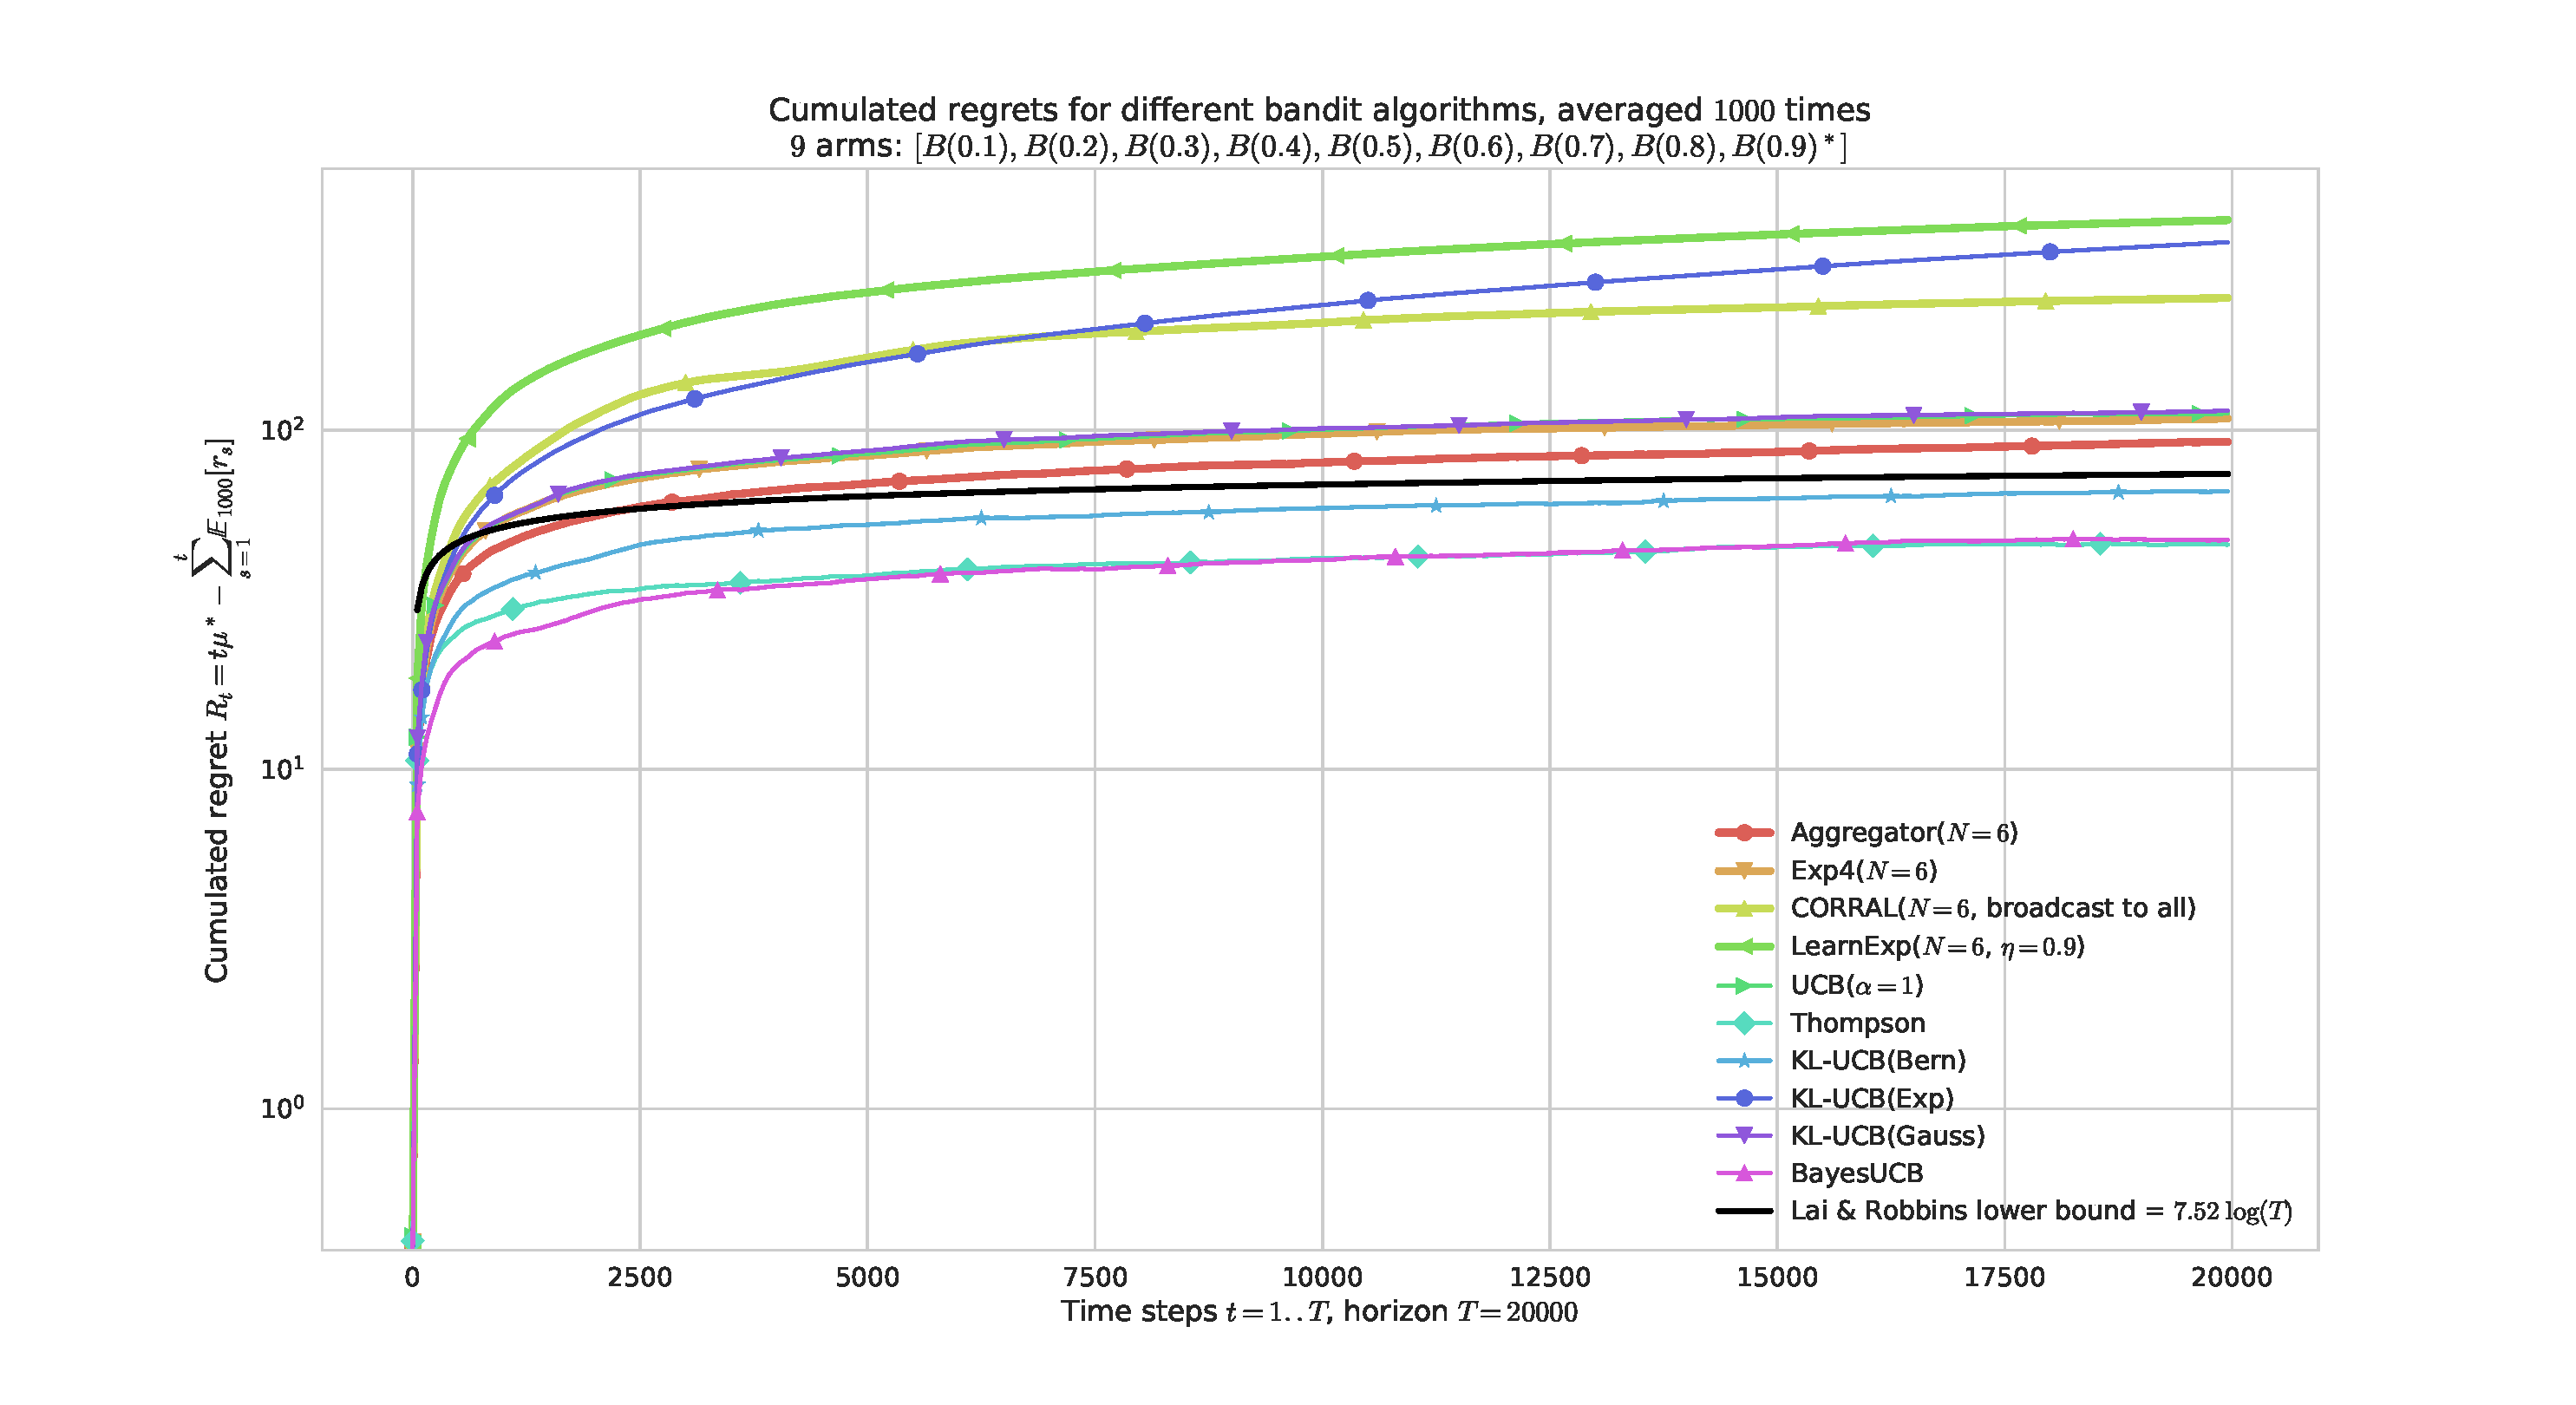
\includegraphics[width=1.10\linewidth]{2-Chapters/2-Chapter/IEEE_WCNC_2018.git/plots/main_semilogy____env1-4_932221613383548446.pdf}
	\caption{On a ``simple'' Bernoulli problem (semilog-$y$ scale).}
	\label{fig:25:EasyBernoulli}
\end{figure}

\begin{figure}[b!]  % [htbp]
	\centering
	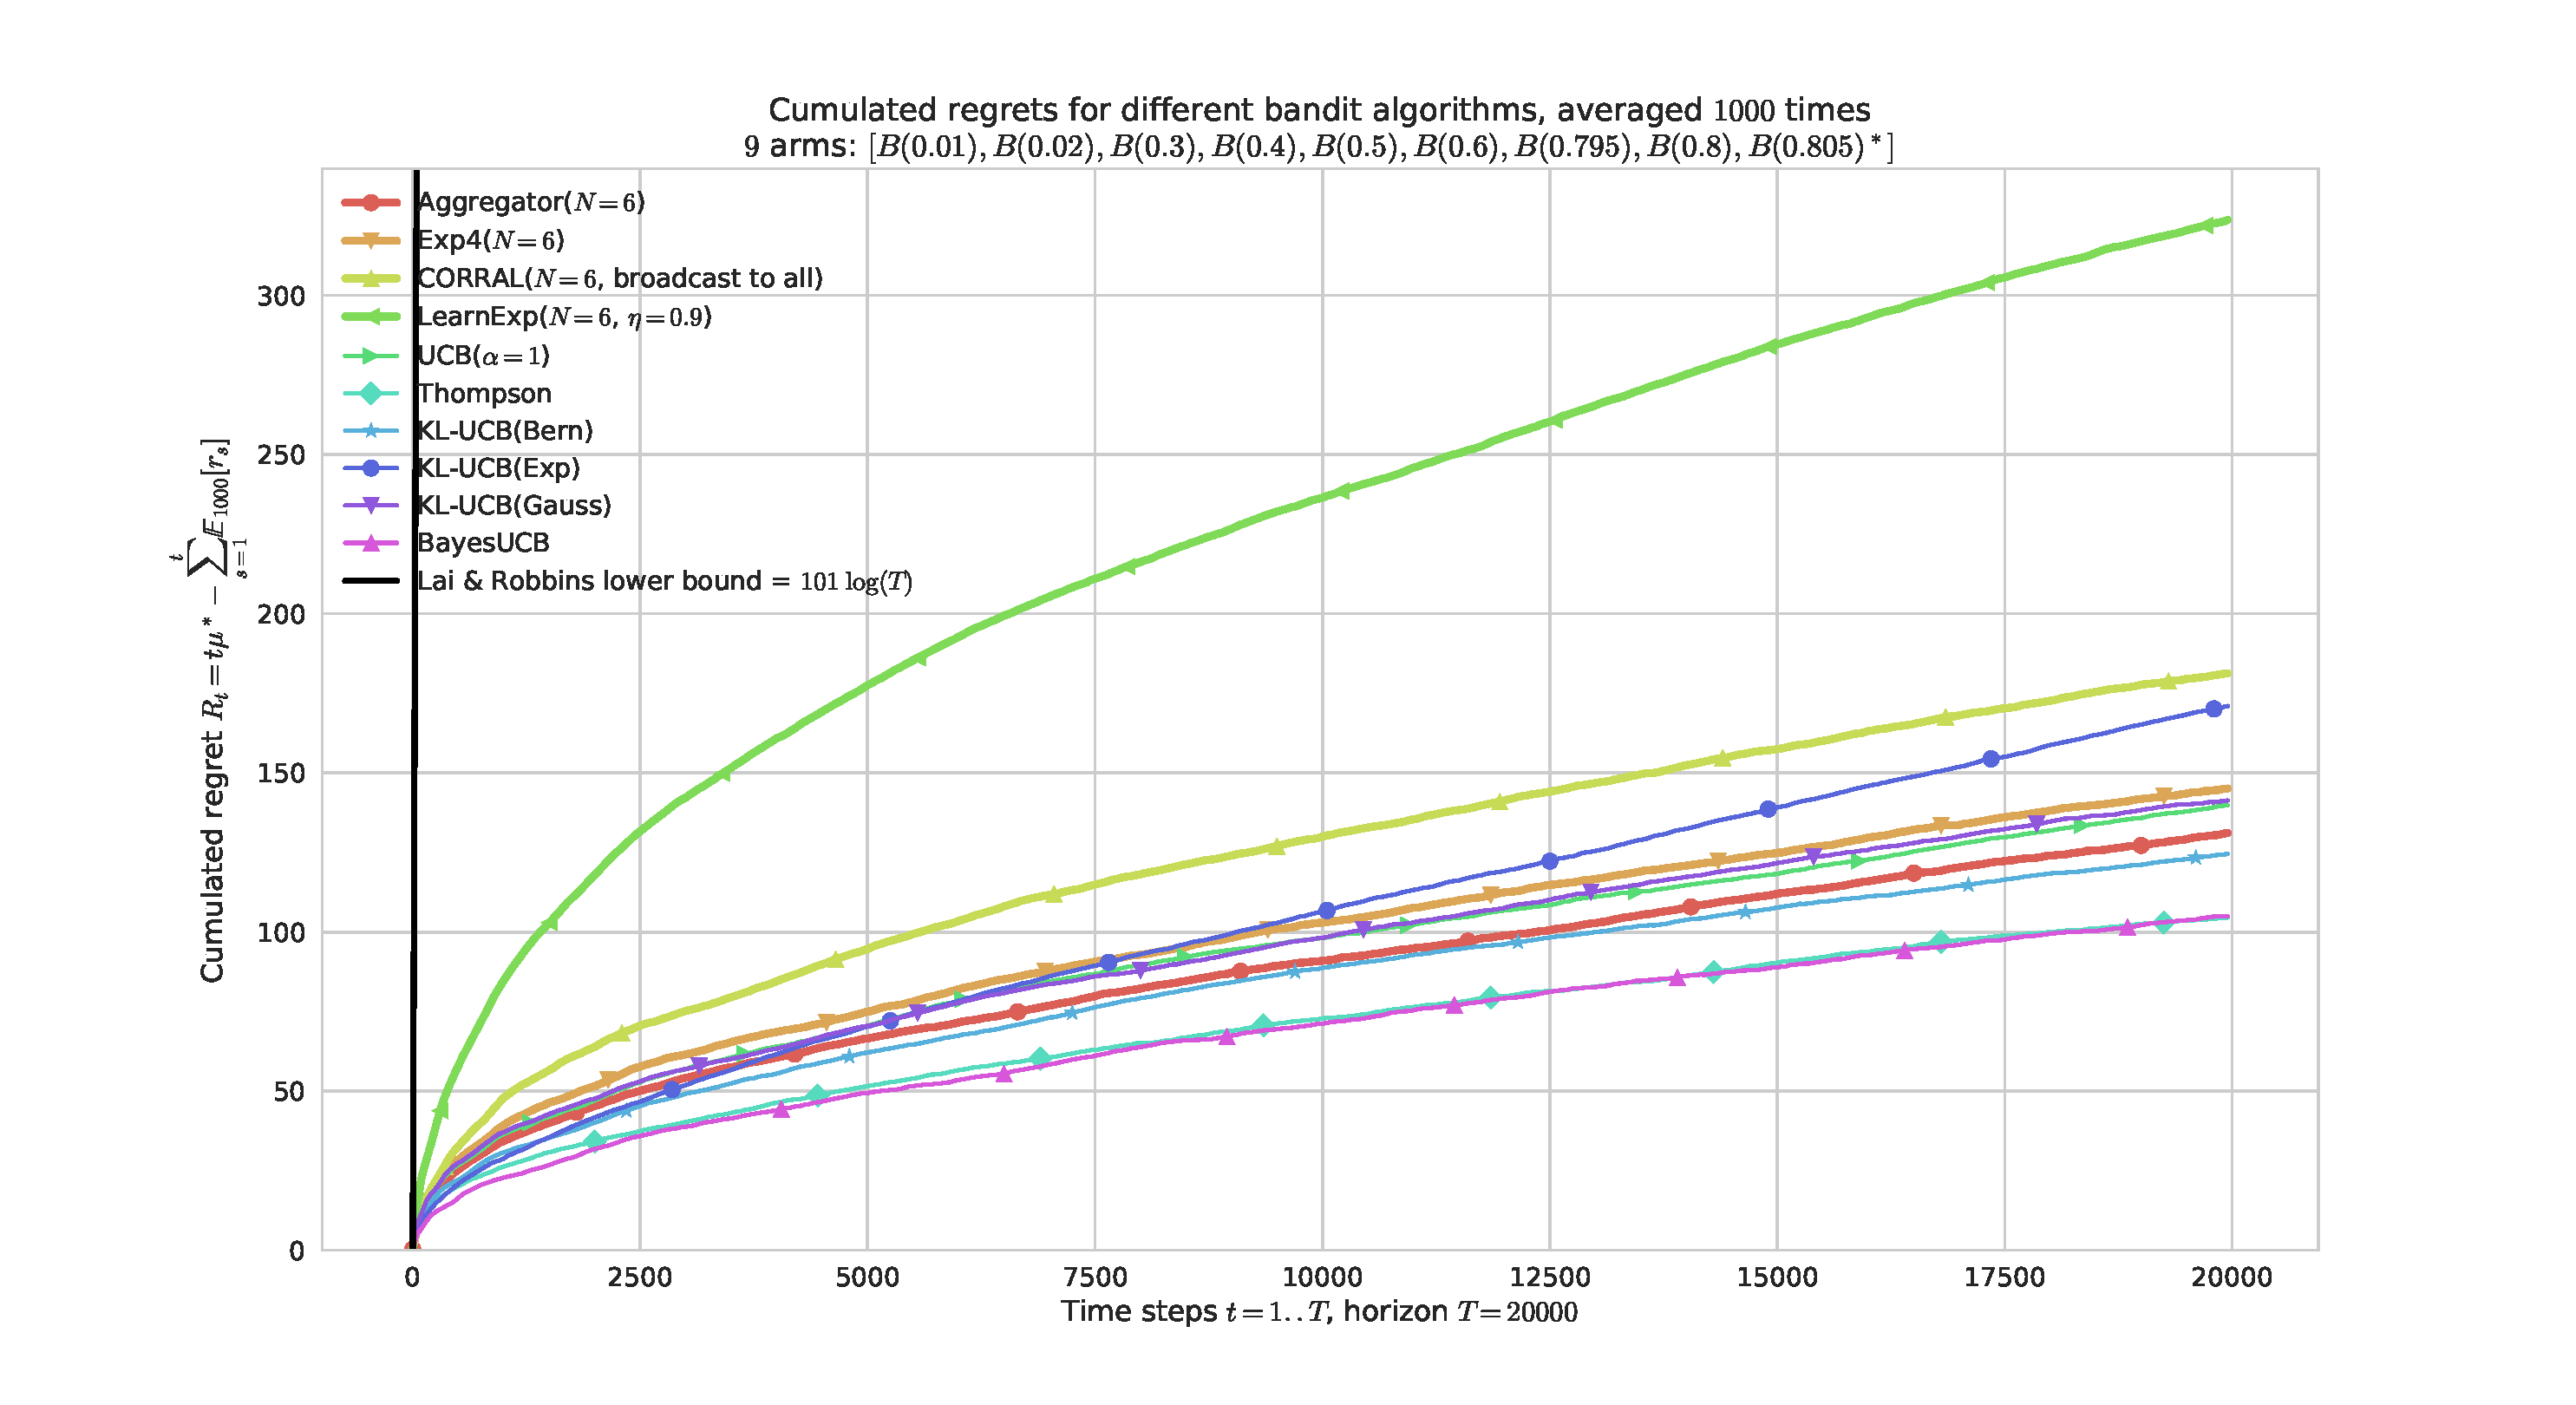
\includegraphics[width=1.10\linewidth]{2-Chapters/2-Chapter/IEEE_WCNC_2018.git/plots/main____env2-4_932221613383548446.pdf}
	\caption{On a ``harder'' Bernoulli problem, they all have similar performances, except \LearnExp.}
	\label{fig:25:HardBernoulli}
\end{figure}

\begin{figure}[b!]  % [htbp]
	\centering
	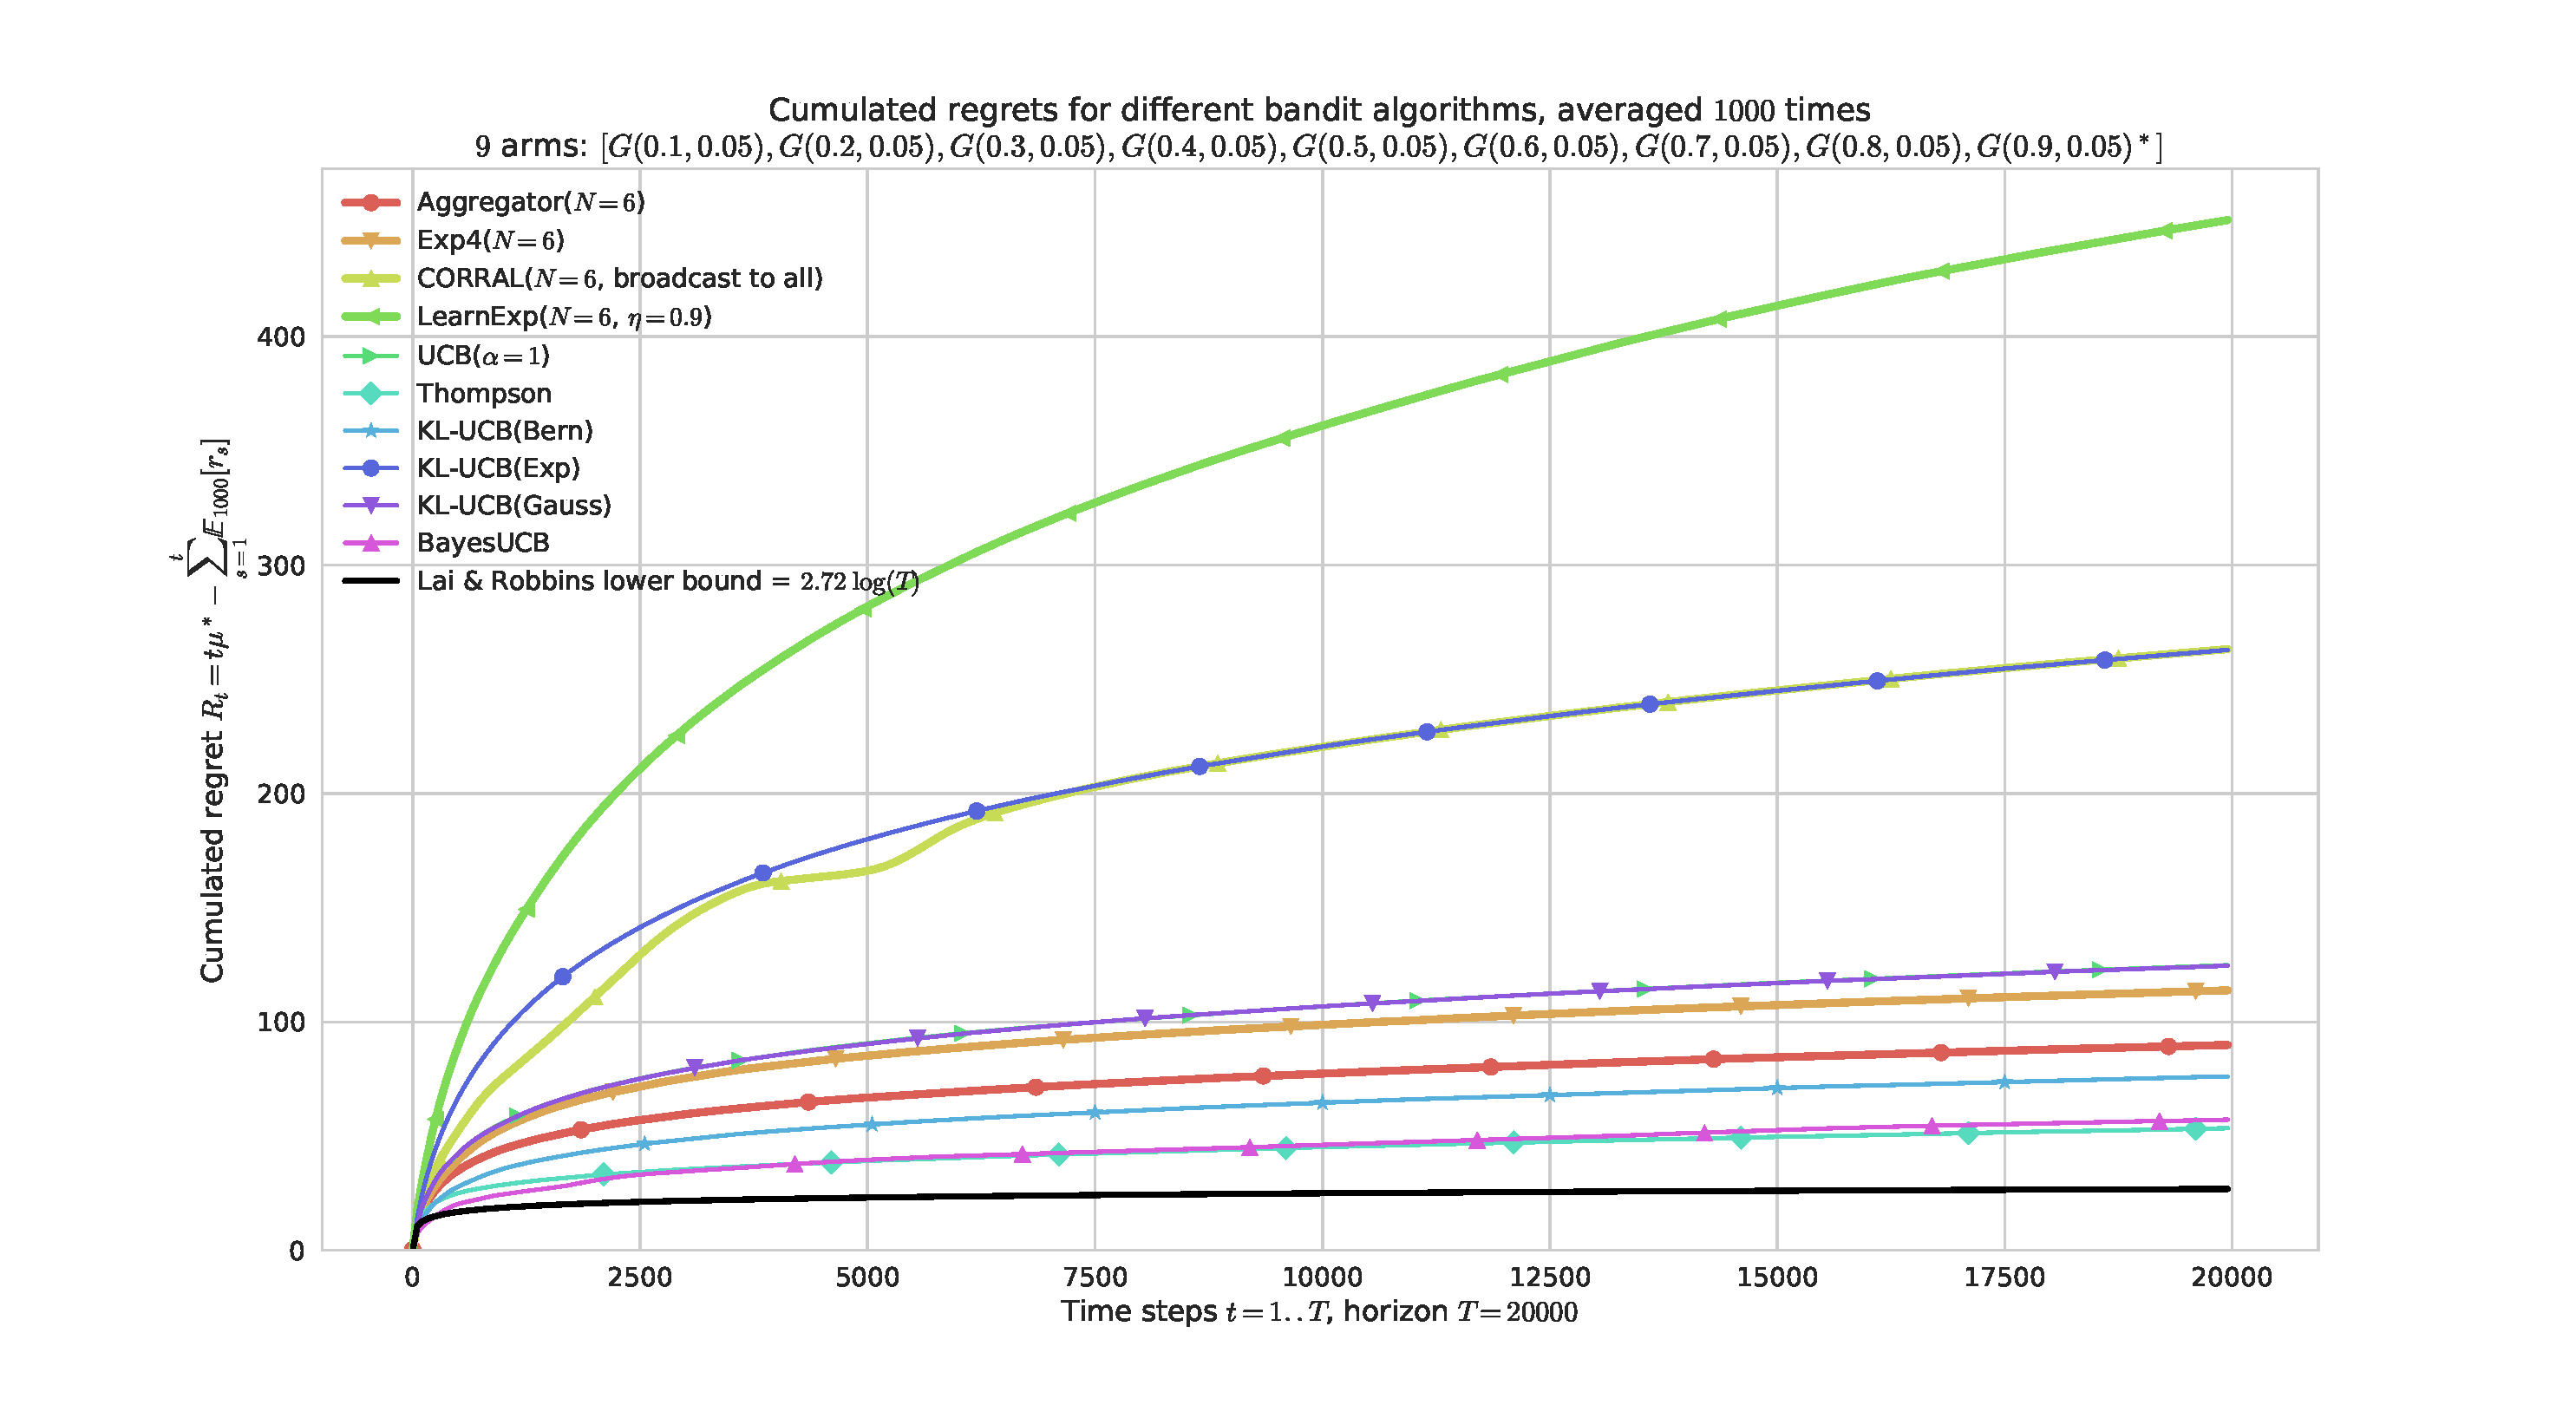
\includegraphics[width=1.10\linewidth]{2-Chapters/2-Chapter/IEEE_WCNC_2018.git/plots/main____env3-4_932221613383548446.pdf}
	\caption{On an ``easy'' Gaussian problem, only \Aggr{} shows reasonable performances, thanks to BayesUCB and Thompson sampling.}
	\label{fig:25:EasyGaussian}
\end{figure}

\begin{figure}[h!]  % [htbp]
	\centering
	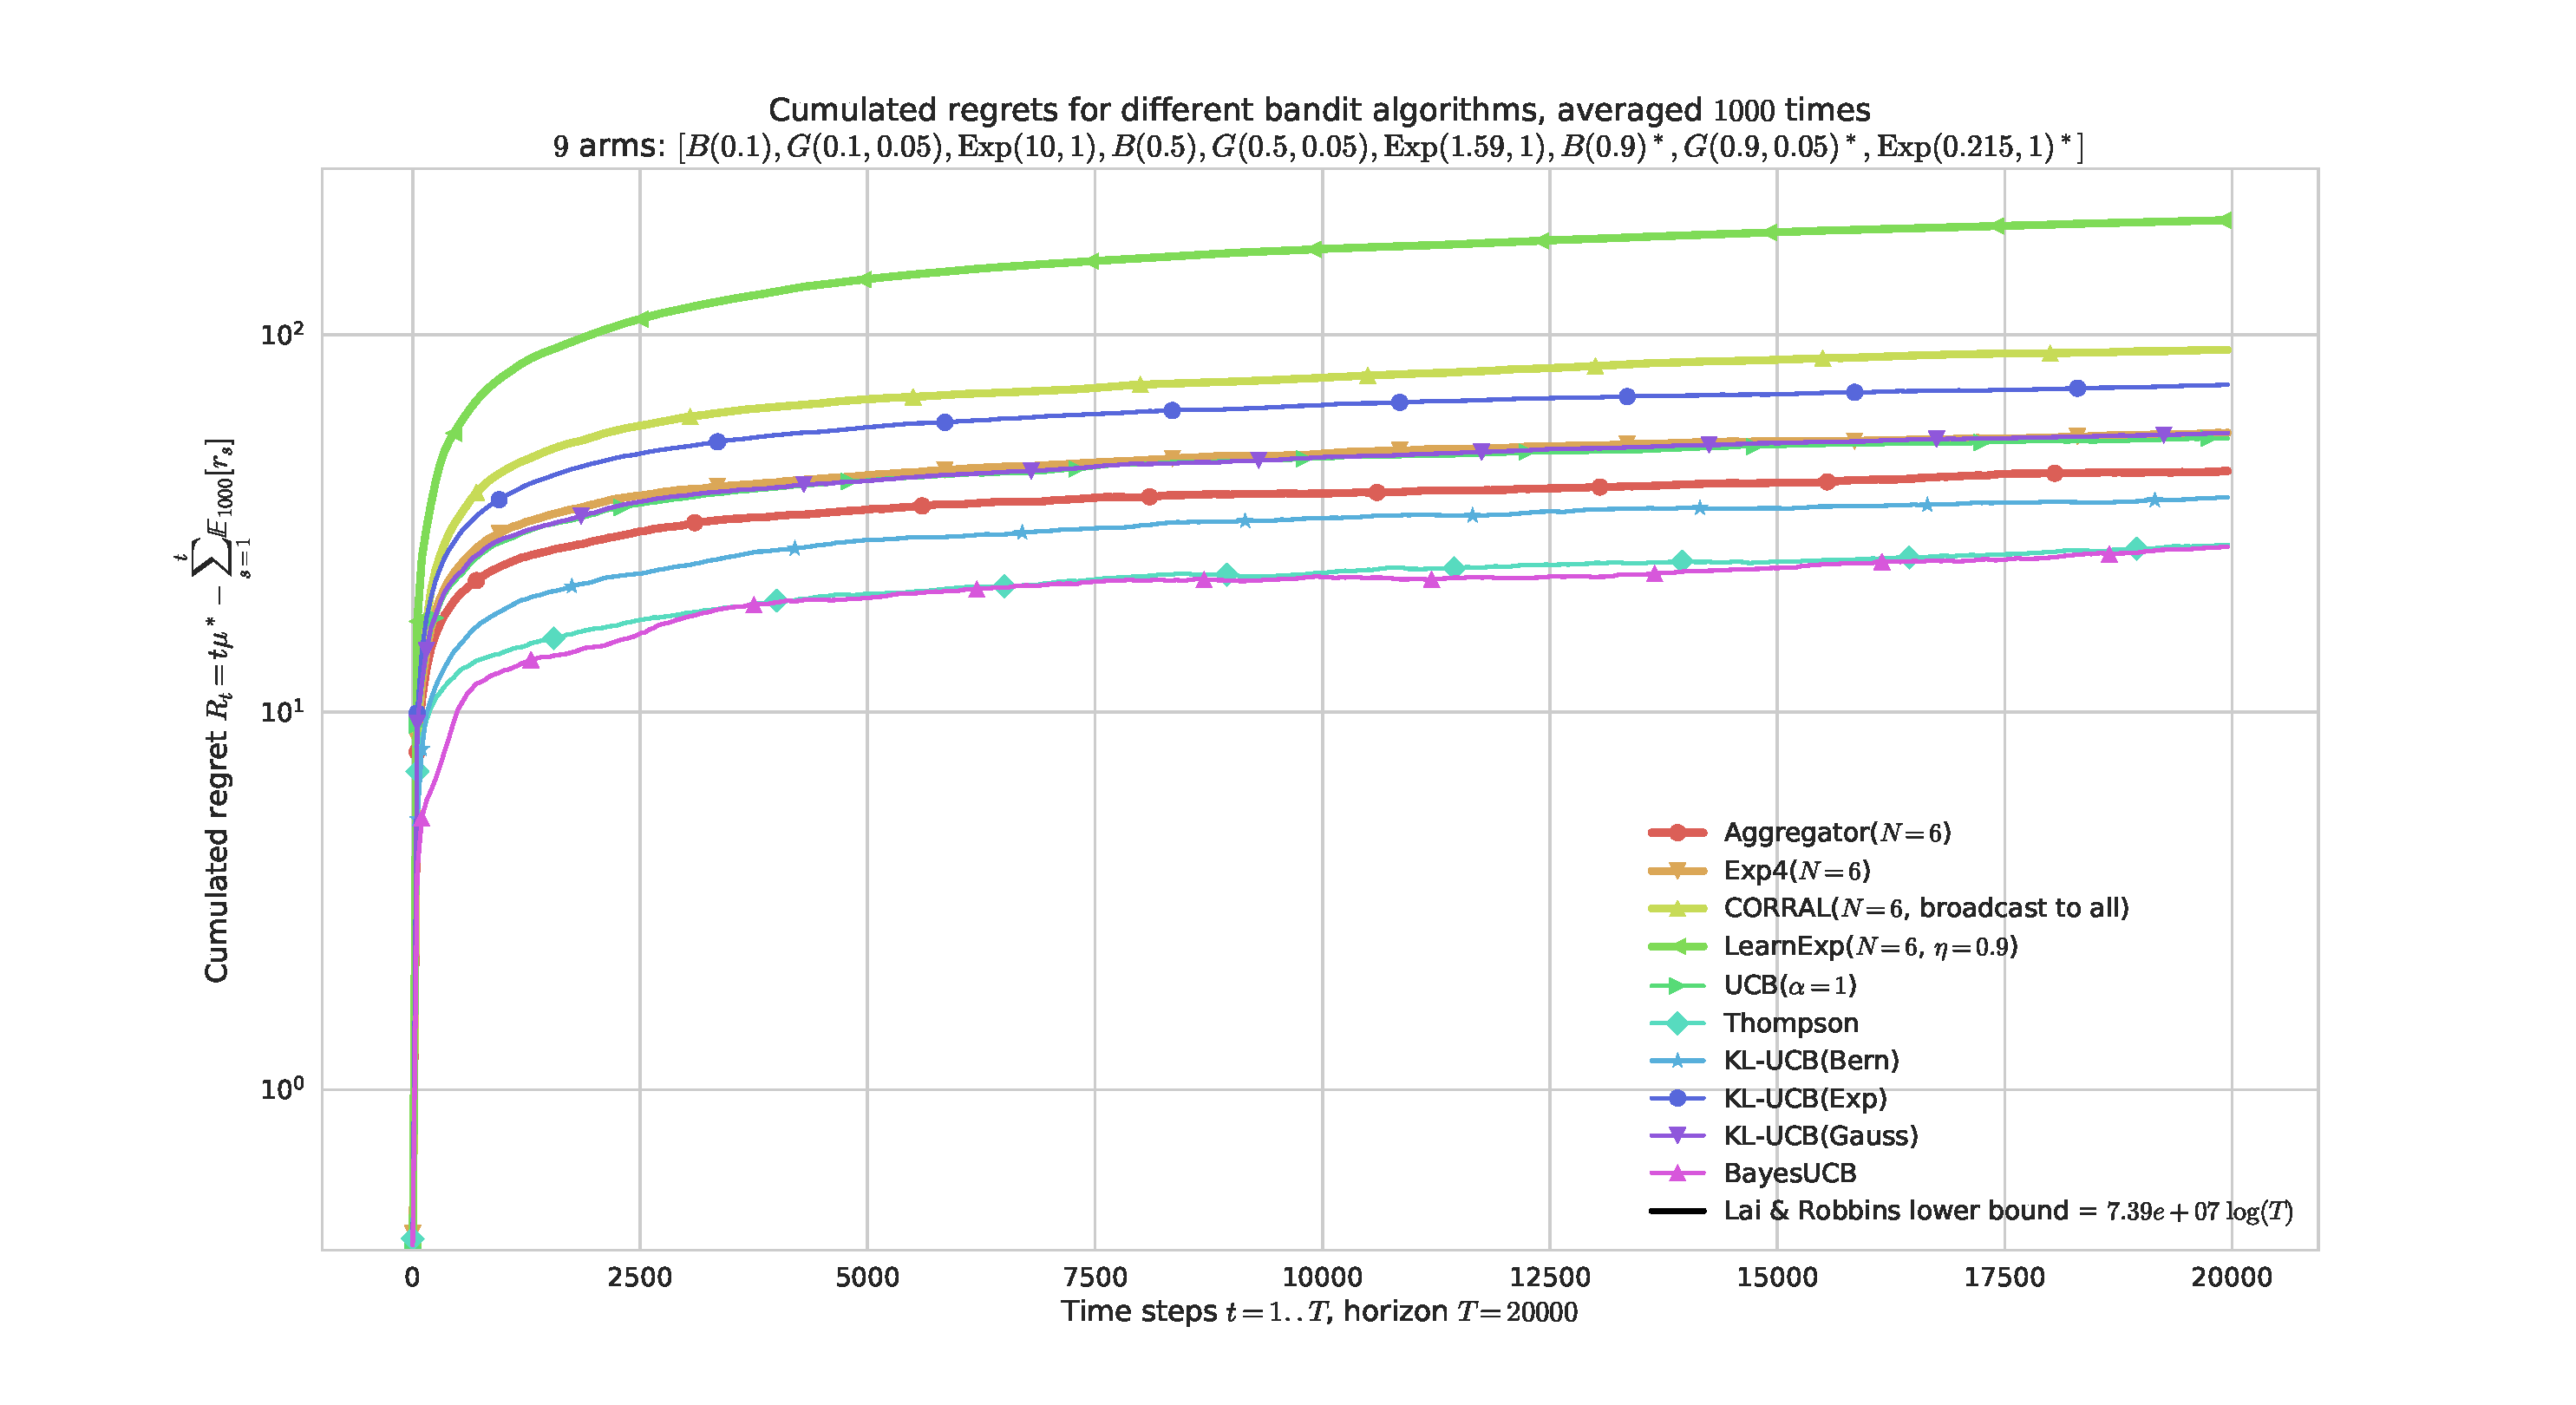
\includegraphics[width=1.10\linewidth]{2-Chapters/2-Chapter/IEEE_WCNC_2018.git/plots/main_semilogy____env4-4_932221613383548446.pdf}
	\caption{On a harder problem, mixing Bernoulli, Gaussian, Exponential arms, with 3 arms of each types with the \emph{same mean}.}
	\label{fig:25:HarderMixed}
\end{figure}

\begin{figure}[b!]  % [htbp]
	\centering
	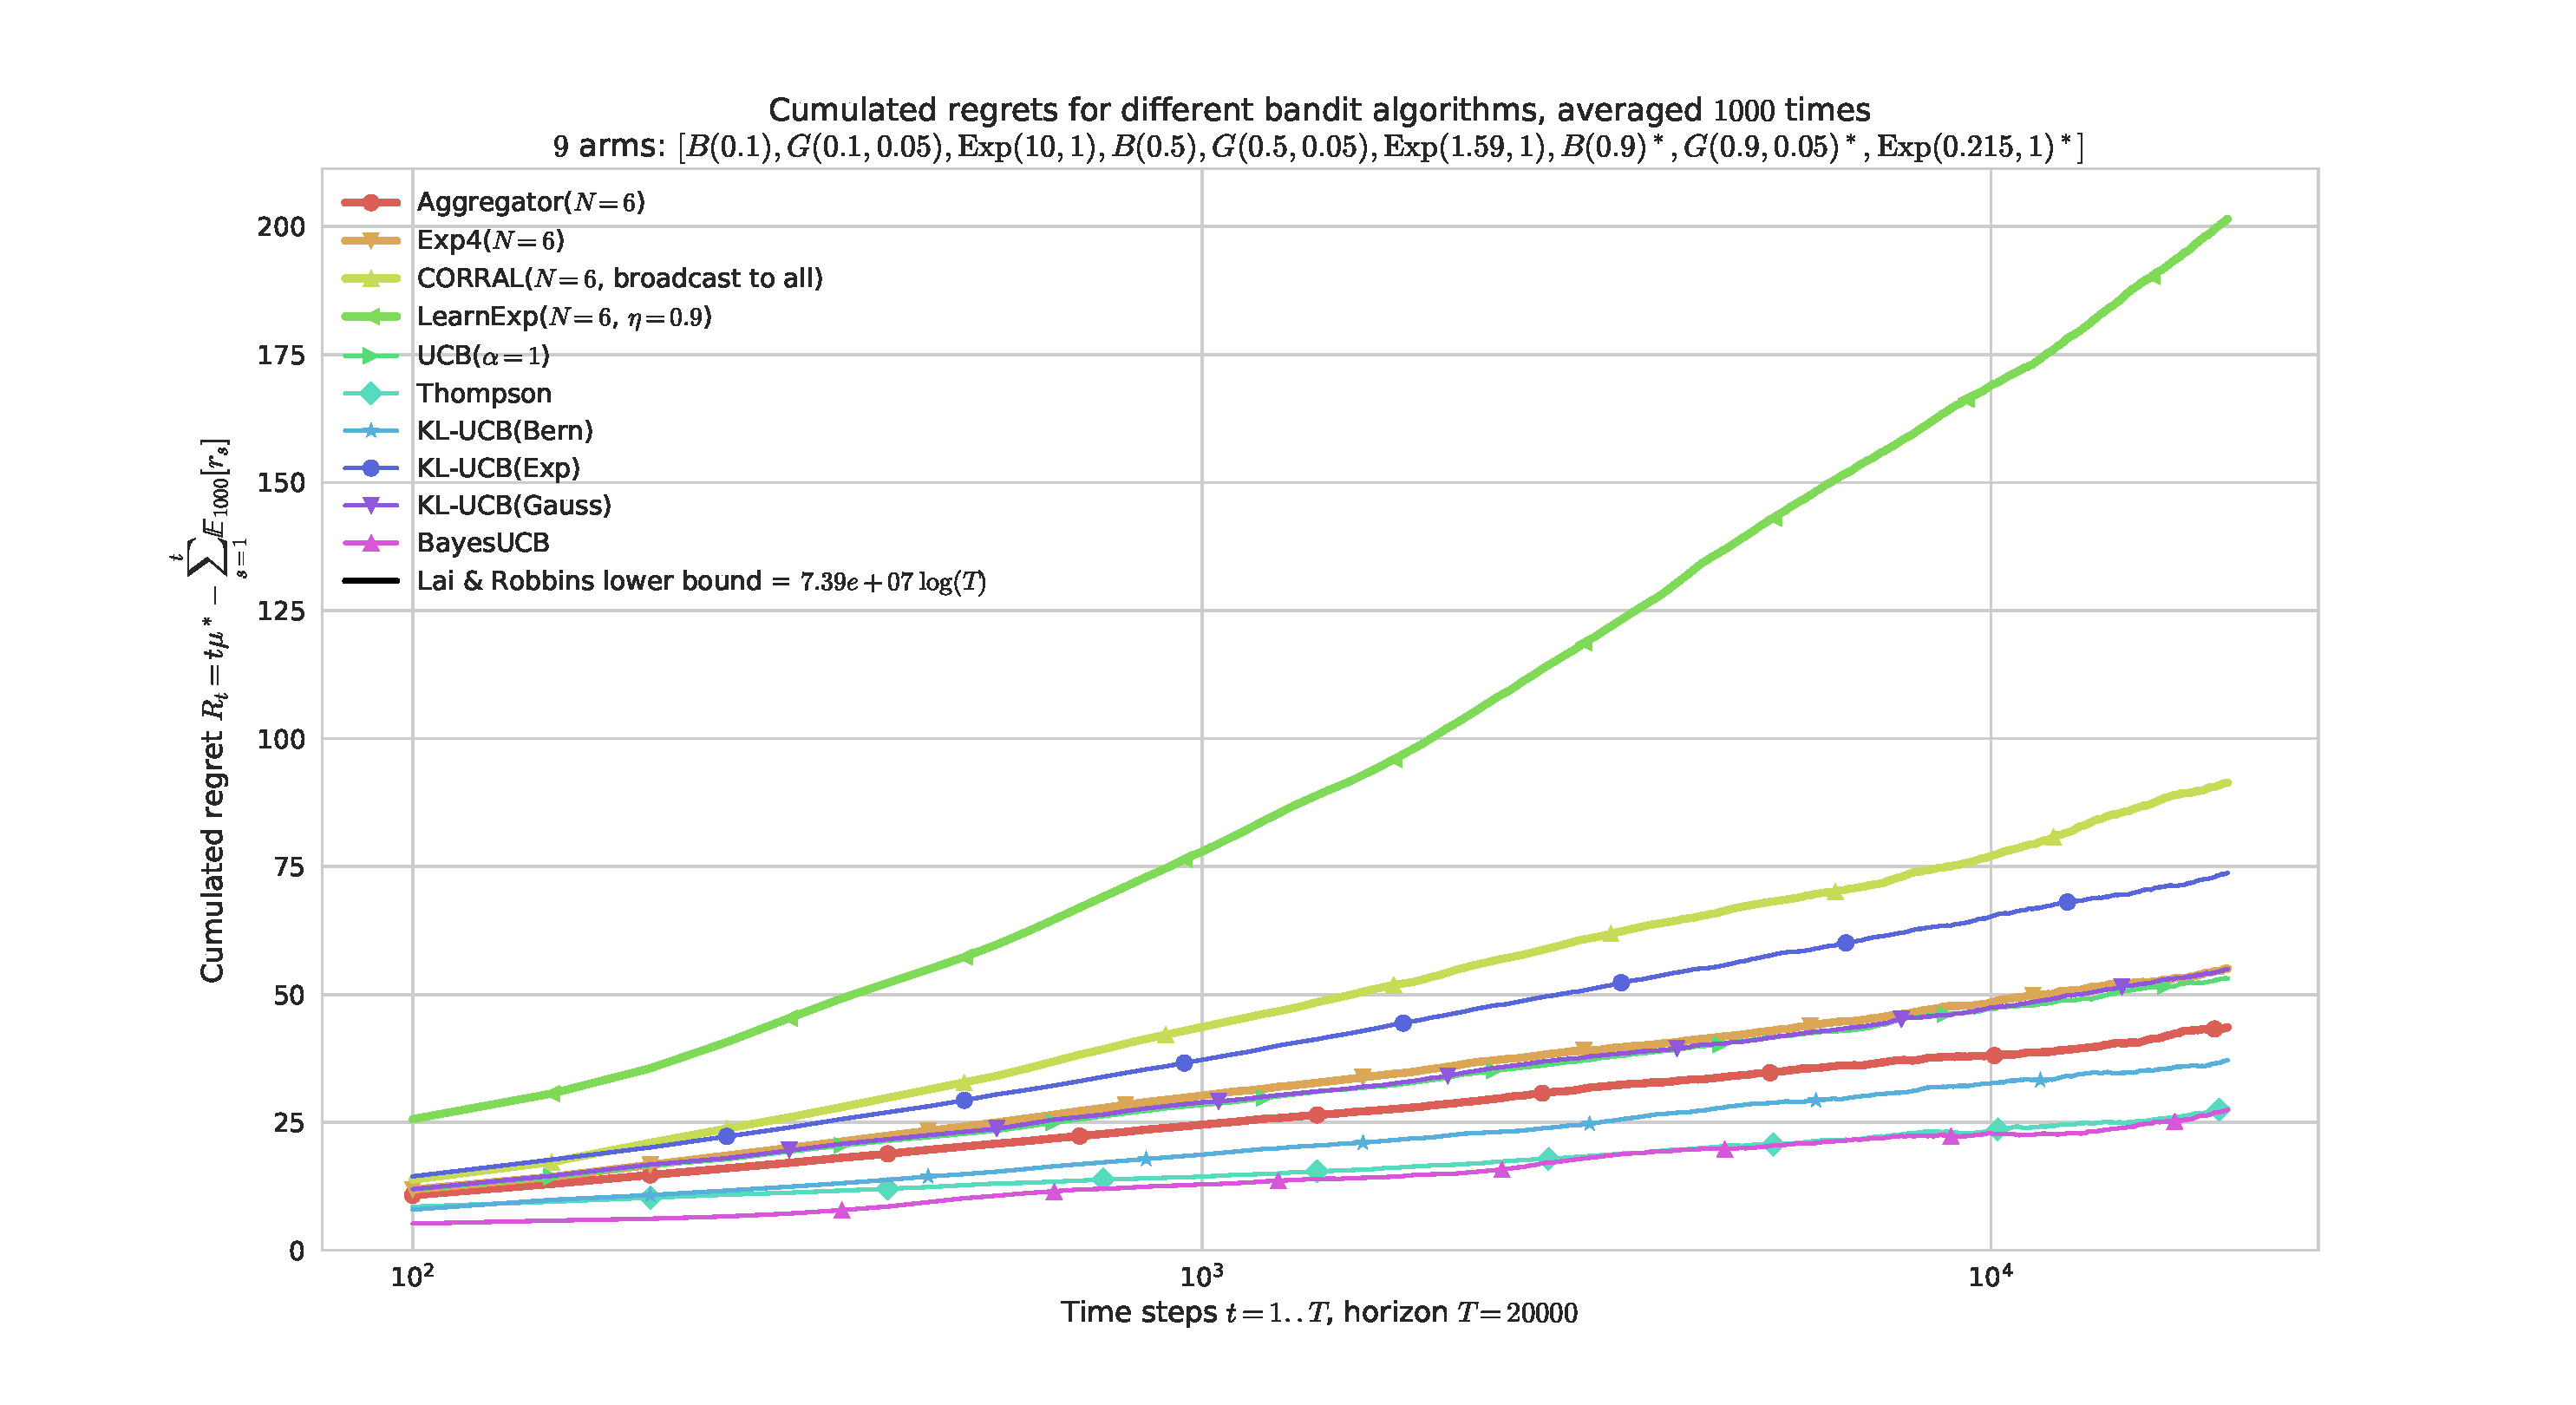
\includegraphics[width=1.10\linewidth]{2-Chapters/2-Chapter/IEEE_WCNC_2018.git/plots/main_semilogx____env4-4_932221613383548446.pdf}
	\caption{The semilog-$x$ scale clearly shows the logarithmic growth of the regret for the best algorithms and our proposal \Aggr, even in a hard ``mixed'' problem (\emph{cf}. Figure~\ref{fig:25:HarderMixed}).}
	\label{fig:25:HarderMixed_semilogx}
\end{figure}

For Bernoulli problems (Figures~\ref{fig:25:EasyBernoulli} and \ref{fig:25:HardBernoulli}), UCB with $\alpha=1/2$, Thompson sampling, BayesUCB and \klUCB{}$^+$ (with the binary $\kl$ function) all perform similarly, and \Aggr{} is found to be as efficient as all of them.
For Gaussian and exponential arms, rewards are truncated into $[0,1]$, and the variance of Gaussian distributions is fixed to $\sigma^2 = 0.05$ for all arms, and can be known to the algorithms (the \kl{} function is adapted to this one-dimensional exponential family).
%
Figure~\ref{fig:25:EasyGaussian} uses only Gaussian arms, with a large gap between their means and a relatively small variance, giving an ``easy'' problem.
%
And Figure~\ref{fig:25:HarderMixed} shows a considerably harder ``mixed'' problem, when the distributions are no longer in the same one-dimensional exponential family and so the Lai \& Robbins' lower-bound no longer holds (even if there still exists a lower-bound).

For each of the 4 problems considered, the \Aggr{} algorithm with default option (broadcast loss to all players) is the best of all the aggregation algorithms,
and its regret is very close to the best of the aggregated algorithms.
Especially in difficult problems with mixed or unknown distributions, \Aggr{} showed to be more efficient that \ExpQ{} and orders of magnitude better than the other reference aggregation algorithms \LearnExp{} and \CORRAL{} (see Figures~\ref{fig:25:HarderMixed} and \ref{fig:25:HarderMixed_semilogx}).


% ----------------------------------------------------------------------
\paragraph{No theoretical guarantees yet}\label{sub:25:theory}

The \Aggr{} does not have satisfying theoretical guarantees in terms of regret $R_T$, unlike many bandit algorithms.
%
Another notion, the \emph{adversarial regret}, denoted by $\overline{R_T}$,
measures the difference in terms of rewards,
between the aggregation algorithm $\Alg_{\mathrm{aggr}}$ and the best aggregated algorithm $\Alg_a$. This is in contrast with the (classical) regret, which measure the difference with the best fixed-arm strategy (Definition~\ref{def:2:regret}).
Thus, even if the aggregated algorithms have logarithmic (classical) regret, having an adversarial regret scaling as $\sqrt{T}$ does not permit to exhibit a logarithmic (classical) regret for the aggregation algorithm.
%
%
Under some additional hypotheses,
\cite[Theorem 4.2]{Bubeck12} proves that
\ExpQ{} satisfies a bound on adversarial regret, % $\overline{R_T}$
$\overline{R_T} \leq 2 \sqrt{T N \log(K)$,
with the good choice of the learning rate sequence $(\eta_t)_{t \geq 1}$.
Our proposed algorithm follows quite closely the architecture of \ExpQ,
and a similar bound for \Aggr{} is expected to hold.
% this is left as a future work.
% For sake of conciseness, we cannot present a proof here.
%

This would be a first theoretical guarantee, but not satisfactory as we saw above that simple algorithms (like \UCB) have regrets scaling as $\log(T)$ \cite{Auer02,Bubeck12}, not $\sqrt{T}$.
%
Regret bounds in several different settings are proved for the \CORRAL{} algorithm \cite{Agarwal16}, but no logarithmic upper-bound can be obtained from their technique, even in the simplest setting of stochastic bandits.
%
However, \Aggr{} always seems to have a (finite-horizon) logarithmic regret in all the experiments we performed,
for both Bernoulli and non-Bernoulli problems (\eg, Gaussian, exponential and Poisson distributions).
Further theoretical developments are left as future work.


% ----------------------------------------------------------------------
\paragraph{Conclusion about our \Aggr{} algorithm}\label{sub:25:conclusion}

We presented the use of aggregation algorithms in the context of Opportunistic Spectrum Access for Cognitive Radio,
especially for the real-world setting of unknown problem instances,
when tuning parameters before-hand is no longer possible and an adaptive algorithm is preferable.
% - \ExpQ and \Aggr works fine
% Both algorithms \ExpQ{} and \Aggr{} have been detailed, and we explained why
Our proposed \Aggr{} was presented in details,
and we also highlighted its differences with \ExpQ.
% as well \color{red} as the intuition that it seems more suited for purely stochastic problems\color{black}.

% - \Aggr{} really help to select the best algorithm against a certain problem, on the fly without any prior knowledge of the problem neither any prior knowledge on which algorithms is the best
We presented experiments on simple MAB problems coming from previous work on bandits for OSA \cite{Jouini10},
and the simulations results showed that \Aggr{} is able to identify on the fly the best algorithm to trust for a specific problem, as expected.
Experiments on problems mixing different families of distributions were also presented, with similar conclusions in favor of \Aggr.
It is not presented in this section, but our proposed algorithm also works well in dynamic scenarios, in which the distribution of the arms can change abruptly at some time,
and appears to be more robust than simple non-aggregated algorithms.

\ExpQ{} has theoretical guarantees in terms of adversarial regret, and even if the same result could hold for \Aggr, results in terms of classical regret are yet to be proved.
Empirically, \Aggr{} showed to always have a logarithmic
regret $R_T$ if it aggregates algorithms with logarithmic regrets (like UCB, \klUCB, Thompson sampling, BayesUCB etc).
It usually succeeds to be close to the best of the aggregated algorithms, both in term of regret and best arm pull frequency.
As expected, the \Aggr{} is never able to outperform any of the aggregated algorithms, but this was an over-optimistic goal.
%
What matters the most is that, empirically, \Aggr{} is able to quickly discover \emph{on the fly} the best algorithms to trust, and then performs almost as well as if it was following it from the beginning.

Our \Aggr{} algorithm could be rewritten as an Online Mirror Descent \cite{Hazan2016introduction,Zimmert2018}, as it is the case for both \ExpQ{} and \CORRAL.
But this direction does not appear very useful, as in the case of \CORRAL{}  the analysis cannot bring a logarithmic regret bound, even by aggregating asymptotically optimal algorithms.
% We will continue investigating regret bounds for \Aggr,
% and other directions include possible applications to the non-stochastic case (\eg, rested or restless Markovian problems, like it was very recently studied in \cite{Luo18}).

\paragraph{Reproducility of the experiments.}
%
Experiments presented in this Section are based on our library SMPyBandits,
and the page \texttt{SMPyBandits.GitHub.io/Aggregation.html} gives instructions to reproduce them.


% ----------------------------------------------------------------------------
% \bibliographystyle{ieeetr}
% \bibliography{IEEE_WCNC__2018__Paper__Lilian_Besson__07-17}


A last solution is online algorithm selection, inspired from expert aggregation.
Include here the discussion about expert aggregation and my \textbf{Aggregator} algorithm, see https://hal.inria.fr/hal-01705292



% ----------------------------------------------------------------------------
\section{Conclusion of Chapter 2}
\label{sec:2:conclusion}

In this chapter, we saw...

Future works include...



% ----------------------------------------------------------------------------
\section{Appendix for Chapter 2}
\label{sec:2:appendix}

\subsection{Eficient numerical computation of Kullback-Leibler divergences and \klUCB{} indexes}

I want to detail the maths behind an implementation of klUCB, see https://smpybandits.github.io/docs/Policies.kullback.html and all what is detailed there.

How to write a fast version of klBern and klucbBern (the two most used functions), using C or Numba or Cython, maybe I can include the speed up simulations here? First piece of code, before really presenting SMPyBandits ?

My work for this part is also published on https://github.com/Naereen/Kullback-Leibler-divergences-and-kl-UCB-indexes
(in Python) and https://github.com/Naereen/KullbackLeibler.jl (in Julia).

